\documentclass[aspectratio=169]{beamer}
\usepackage{graphicx,tikz,pgfpages}
\setbeamertemplate{navigation symbols}{}
\ifdefined\presenternotes\setbeameroption{show notes on second screen=right}\else\setbeameroption{hide notes}\fi
\begin{document}
\begin{frame}[plain]
\begin{tikzpicture}[remember picture,overlay]\node at (current page.center) {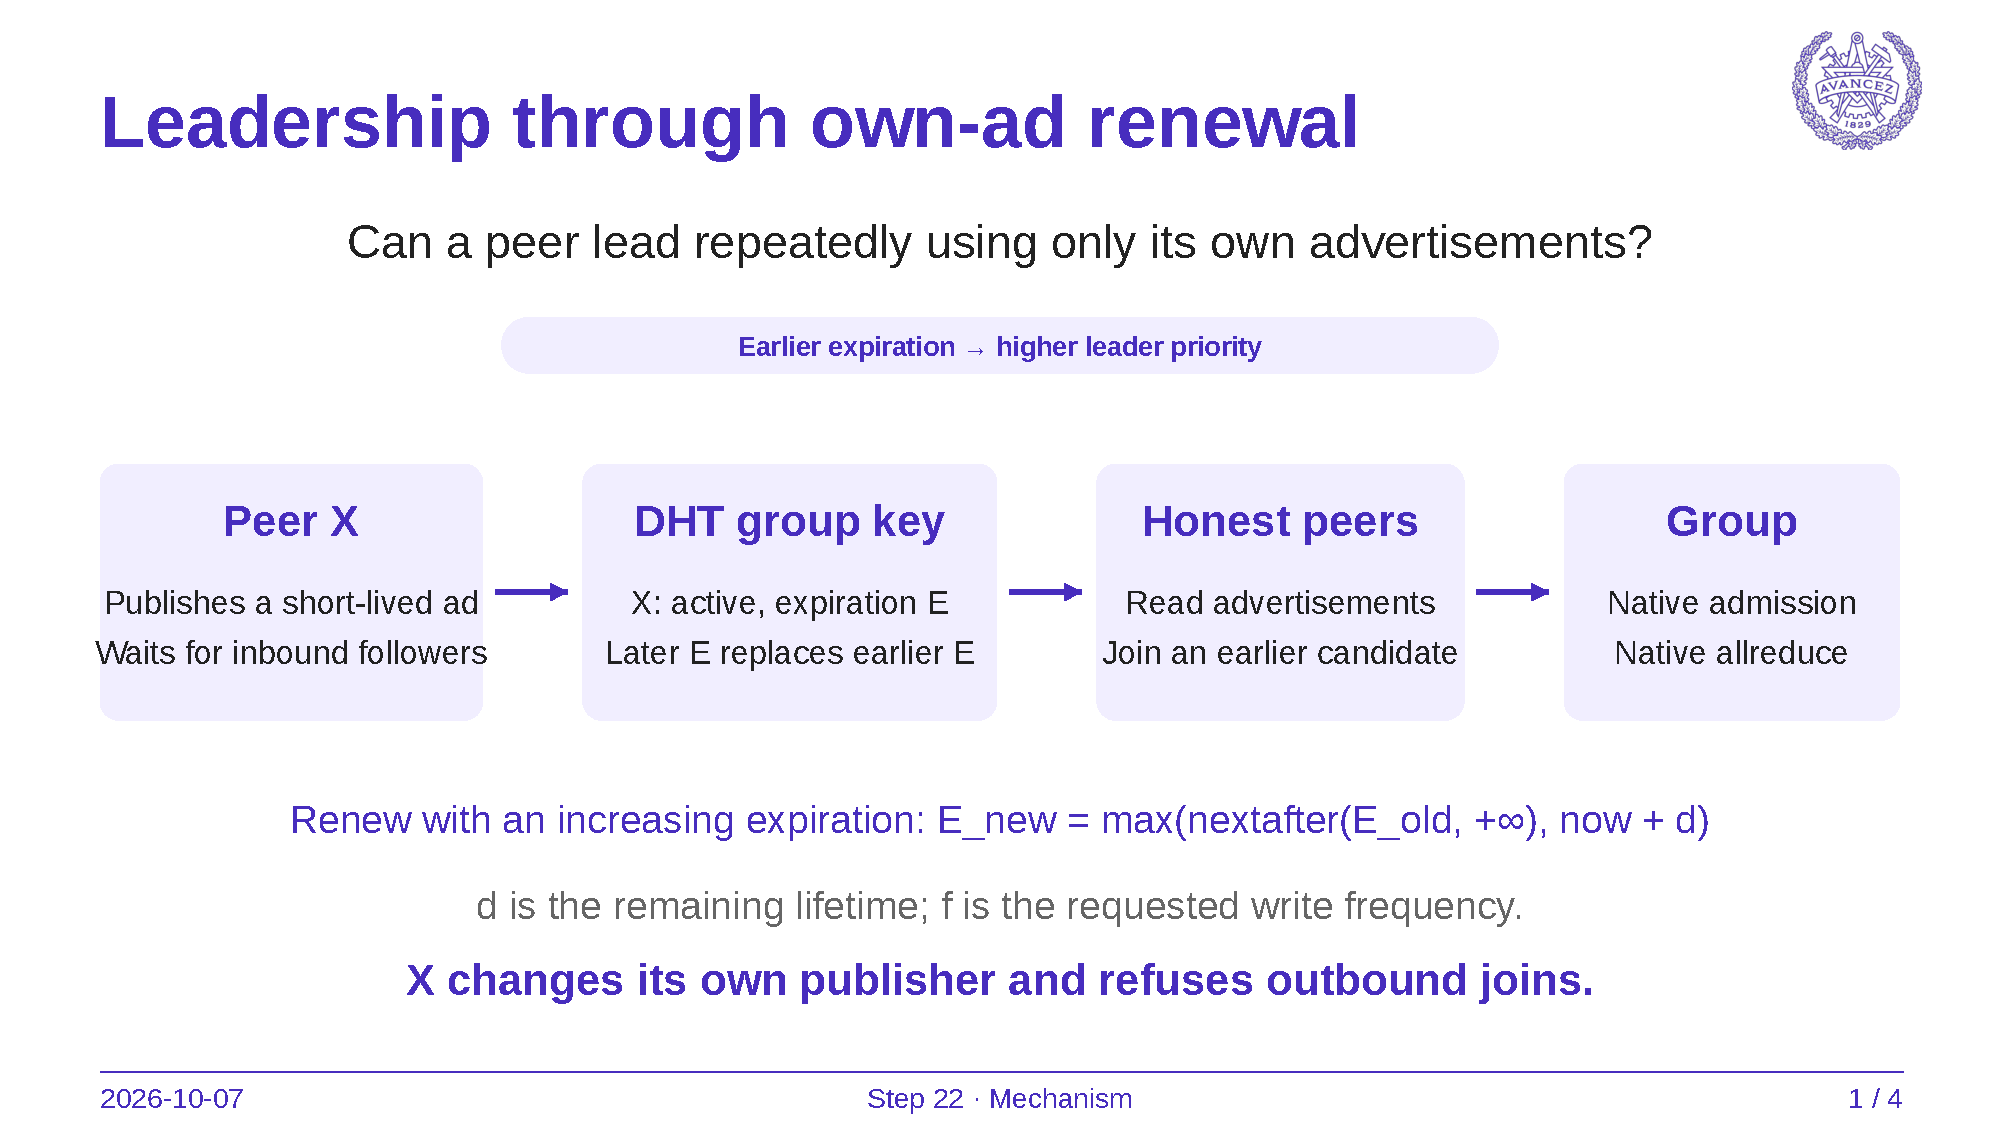
\includegraphics[width=\paperwidth,height=\paperheight]{slides/01.pdf}};\end{tikzpicture}
\note{Step 22 tests a different policy from adaptive undercutting. X does not read competitor advertisements through the matchmaking API and does not forge another peer's records. Its publisher uses a short remaining lifetime d, renews at requested frequency f, and waits for inbound followers. The harness retains the stock admission checks and allreduce.

Hivemind stores availability under the group key and a PeerID subkey. The expiration serves both as the record lifetime and as leader priority. Peers prefer an earlier (expiration, PeerID-bytes) tuple, while a holder only replaces an existing record when the incoming expiration is strictly greater. The publisher therefore uses E\_new = max(nextafter(E\_old, +infinity), now + d), capped at the current search deadline. It never declares a remaining lifetime above five seconds. A renewal normally advances E by approximately one send period; it does not keep priority fixed. Requested frequency can exceed achieved frequency when stores serialize.

For overlapping holder visibility, d > 1/f + write latency + jitter margin is a useful condition, not a leadership guarantee. DHT positions are ordinary seeded positions, not crafted identities. Sources: publisher, repository `hivemind/averaging/key\_manager.py`, `hivemind/utils/timed\_storage.py`, and `hivemind/averaging/matchmaking.py`. The diagram shows logical decisions, not measured packet timing.}
\end{frame}
\begin{frame}[plain]
\begin{tikzpicture}[remember picture,overlay]\node at (current page.center) {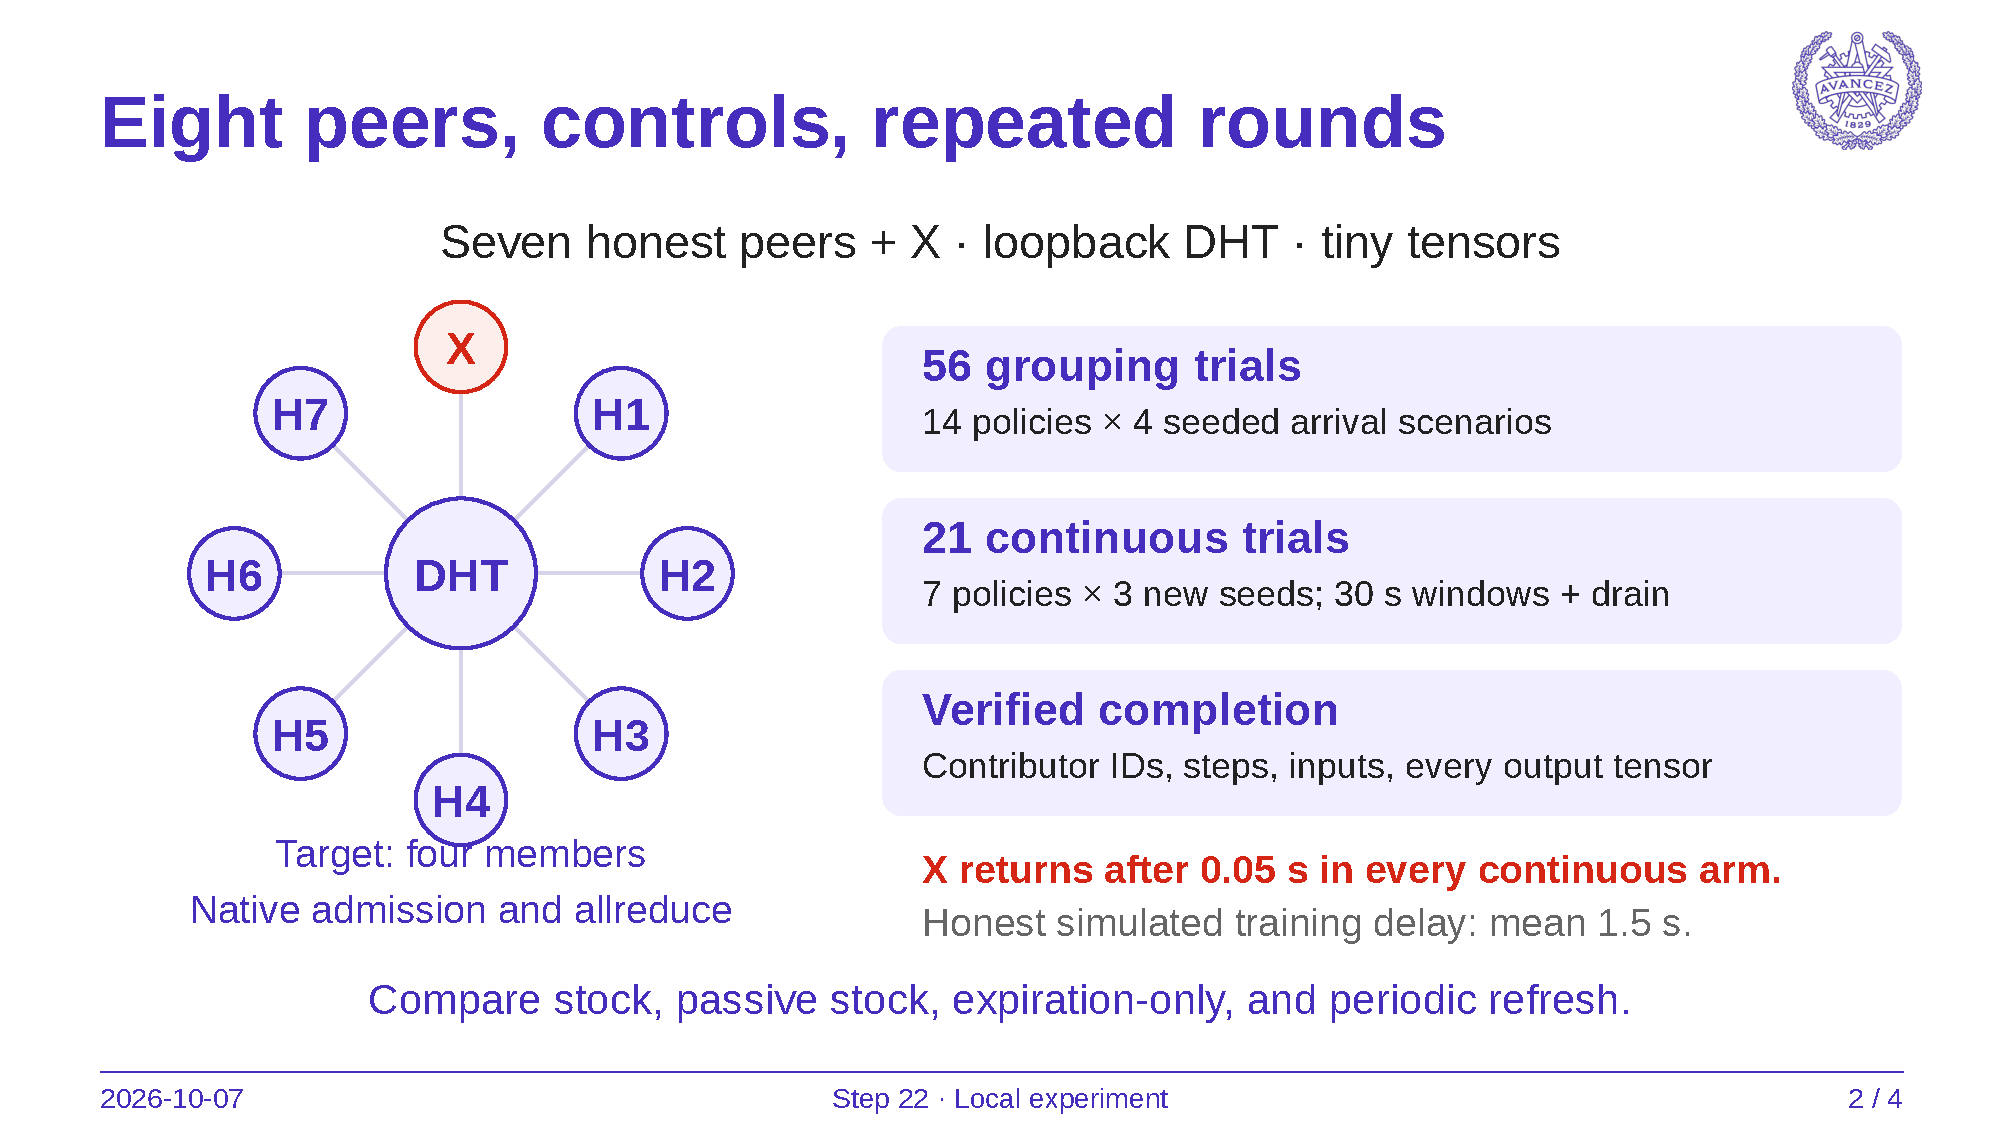
\includegraphics[width=\paperwidth,height=\paperheight]{slides/02.pdf}};\end{tikzpicture}
\note{All trials are private eight-peer loopback experiments with standalone DecentralizedAverager instances and 128-element tensors. They are not full Optimizer training. There is no explicit scheduled\_time. Honest peers have the default five-second matchmaking window, a two-member minimum, and a three-second join-request timeout. The target is four. Each step has a twelve-second matchmaking limit and a six-second allreduce limit. Empty group bits keep repeated steps under the same group key. Core Hivemind source is unchanged.

The grouping wave uses two seeds (2202, 2203) with staggered and bursty arrivals: four scenarios per policy, fresh networks per trial. X starts independently over three seconds. In this sweep the stock control has a two-member minimum and may follow; the passive control refuses outbound joins and has minimum four. All 56 final trials returned correct tensors; one honest step did not find a group. The 0.5/s, d=2.085764 s policy led 4/4 scenarios using five active ad writes; both controls led 3/4. These are small counts, not deployment success rates.

Continuous trials use held-out seeds 2211-2213. New submissions last thirty seconds and already submitted steps then drain. X has minimum four in every continuous arm, including stock. Honest re-entry delays are lognormal with mean 1.5 s, coefficient of variation 0.6, clipped to 0.1-4 s. X returns after 0.05 s in every arm. That fast re-entry gives X more opportunities and prevents interpreting these counts as an ad-only advantage over equally paced peers. The output check matches contributor identities, step numbers, input values, and every member's tensor; a successful future is insufficient. See the full methods and exact tables in the notes appendix.}
\end{frame}
\begin{frame}[plain]
\begin{tikzpicture}[remember picture,overlay]\node at (current page.center) {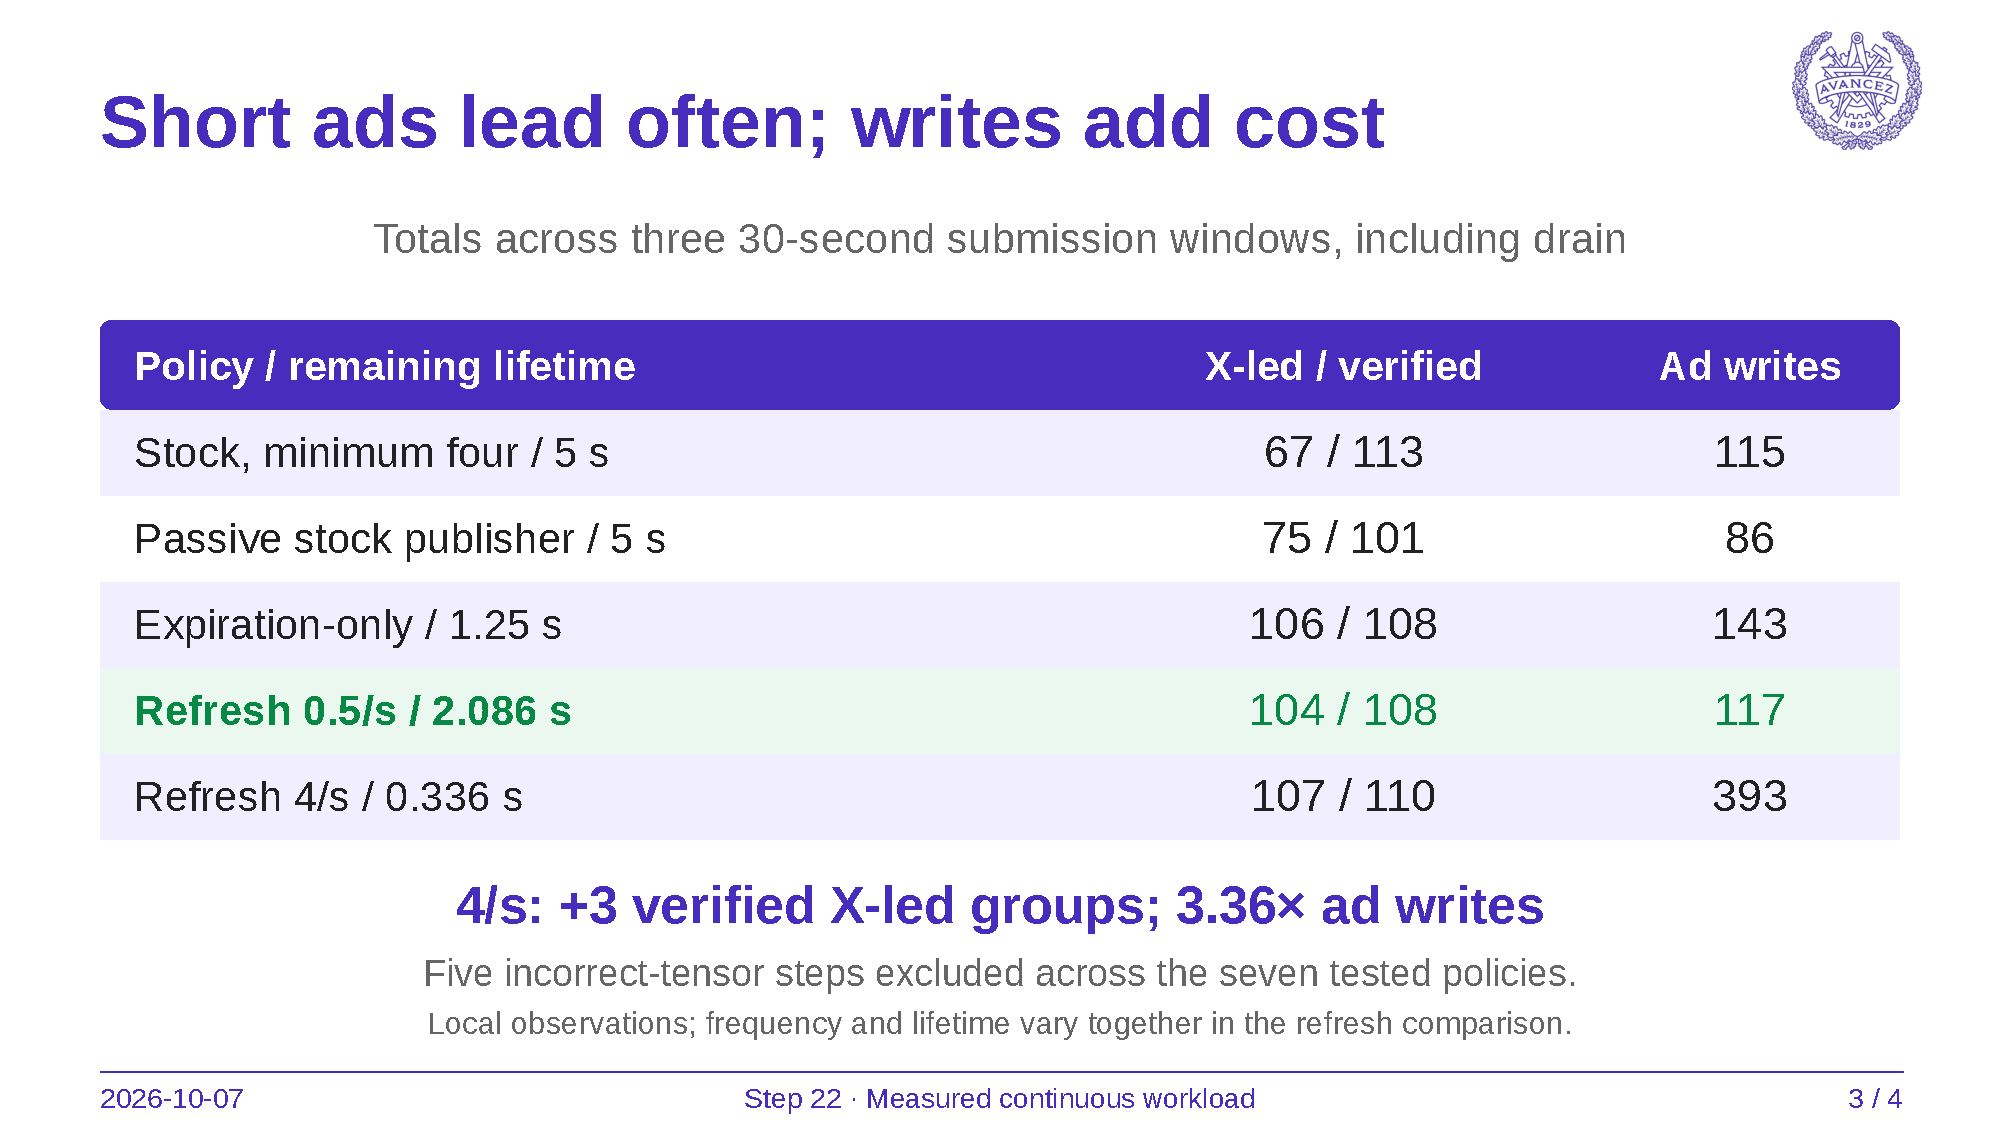
\includegraphics[width=\paperwidth,height=\paperheight]{slides/03.pdf}};\end{tikzpicture}
\note{The table selects the controls, expiration-only alternative, and the lowest and highest tested refresh frequencies. The full seven-policy table is in the appendix. Numerators are verified X-led groups; denominators are all verified groups in that policy's three runs. These are accumulated observations including drain after the thirty-second submission windows, not requests per second or estimated long-run probabilities.

The 0.5/s policy produced 104 verified X-led groups with 117 active ad writes; 4/s produced 107 with 393 writes, a 3.36-fold write count. Three extra groups across three seeds do not establish a repeatable gain. Frequency and lifetime both change, so this is not a causal estimate of frequency alone. Expiration-only 1.25-second ads produced 106 verified X-led groups with 143 writes; periodic overlap is therefore not necessary for high observed leadership counts in this workload. Its purpose is record continuity, a distinct property.

Five completed steps returned incorrect tensors: one in 0.5/s, three in 1/s, and one in 2/s. Groups containing these steps were excluded from the verified-group counts. The traces establish the errors but do not establish their cause or a causal link to advertisement policy. No forbidden X competitor reads or outbound joins occurred. Writes count high-level active ad attempts, excluding withdrawals, DHT routing walks and other traffic; bytes were not measured. Evidence: continuous raw traces, analysis.}
\end{frame}
\begin{frame}[plain]
\begin{tikzpicture}[remember picture,overlay]\node at (current page.center) {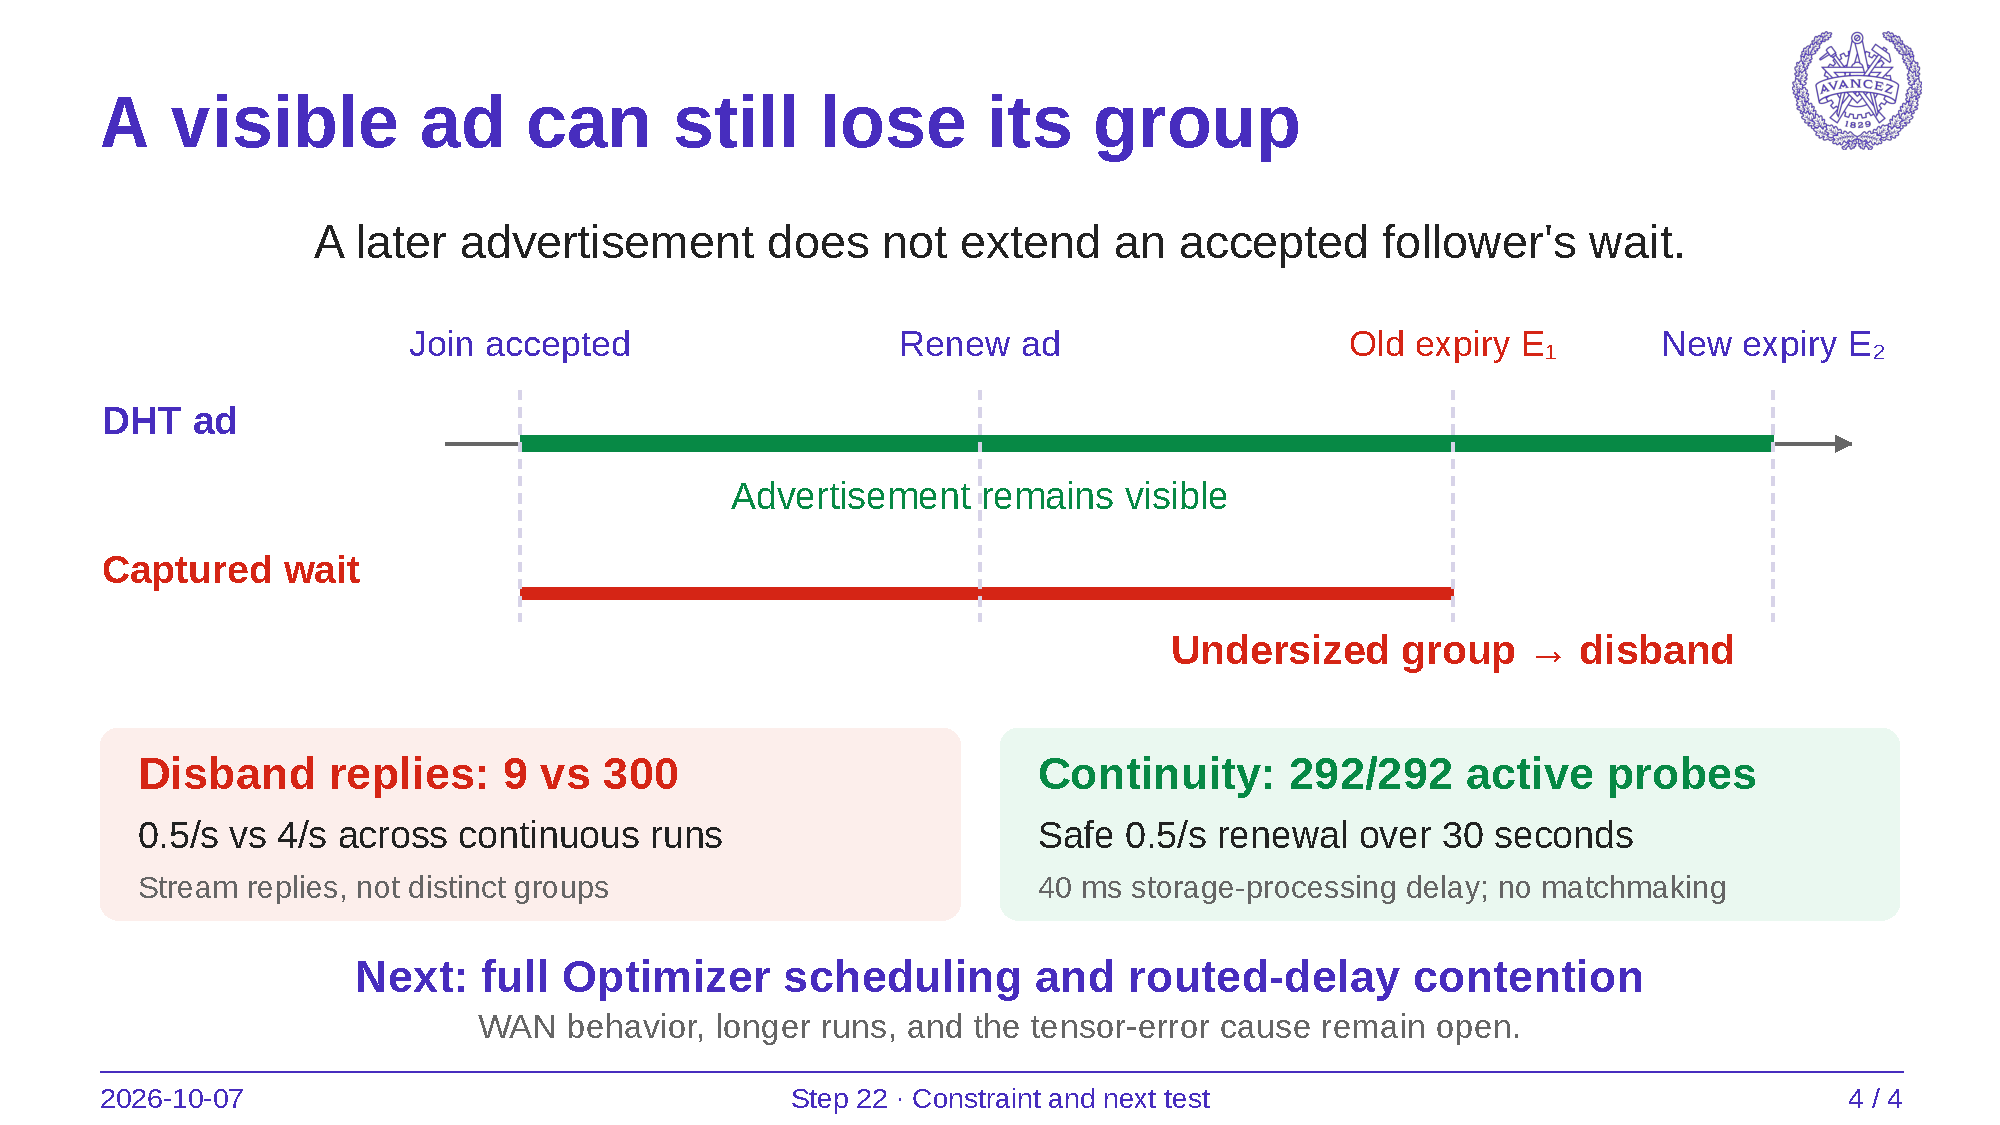
\includegraphics[width=\paperwidth,height=\paperheight]{slides/04.pdf}};\end{tikzpicture}
\note{The timeline is schematic. In rpc\_join\_group, after ACCEPTED, the native leader handler computes a wait timeout from its current declared expiration once. Later publisher renewals do not replace that already captured timer. When the earlier timer fires, the leader can assemble if its native minimum is met; otherwise it can disband an undersized group despite a renewed DHT advertisement. Setting target at least minimum is necessary because the target-size assembly path otherwise bypasses the minimum-size timeout check.

The continuous 4/s policy emitted 300 GROUP\_DISBANDED replies, versus nine at 0.5/s. These are replies on join streams, not counts of unique groups. The comparison also varies remaining lifetime and reflects this local workload; faster writes did not reliably cure assembly churn.

Persistence is a separate record-visibility test: fixed 40 ms remote rpc\_store processing delay, eight DHT peers, independent latest=True probes every 0.1 s, thirty seconds of own-ad writes, no matchmaking. Safe 0.5/s renewal was active at 292/292 probes; safe 2/s at 295/295. A 2/s control with d=0.2 s was active at only 80/295 probes despite 60/60 accepted writes. This is storage-delay emulation, not WAN-delay emulation or proof of indefinite availability. Interior holder intervals exclude local self-stores, initial propagation and final expiration.

A separate capability check with native minimum five and target five formed nine verified X-led five-member groups on one seed during a twelve-second submission window plus drain; 36/37 honest steps completed correctly. It establishes feasibility in that setup, not assured assembly. Next tests should restore full Optimizer-driven epoch scheduling and then add routed delays under controlled conditions. Longer-run behavior, WAN loss/churn, and the five incorrect-tensor steps remain unresolved. Source: repository `hivemind/averaging/matchmaking.py` around rpc\_join\_group; persistence traces, five-member traces.}
\end{frame}
\end{document}
